\documentclass[a4,12pt]{article}
\usepackage[a4paper]{geometry}
\usepackage{graphicx}
\usepackage{pict2e}
\usepackage{xcolor}
\usepackage{subcaption}
\usepackage{amsfonts}
\usepackage{amsmath}
\usepackage{amssymb}
%\usepackage{epstopdf}
\usepackage[backend=bibtex,style=ieee]{biblatex}
\addbibresource{ww.bib}


\newcommand{\fww}[0]{\mathcal{F}^{\mathrm{WW}}}
\newcommand{\fdp}[0]{\mathcal{F}^{\mathrm{dipole}}}
\newcommand{\sdp}[0]{\sigma_{\mathrm{dipole}}}
\newcommand{\sdpa}[0]{\sigma_{\mathrm{dipole\,Adj.}}}
\newcommand{\GeV}[0]{\mathrm{GeV}}
\newcommand{\comment}[1]{\texttt{\color{red}#1}}

\begin{document}
	\begin{figure}[t]
		\begin{subfigure}{0.5\textwidth}
			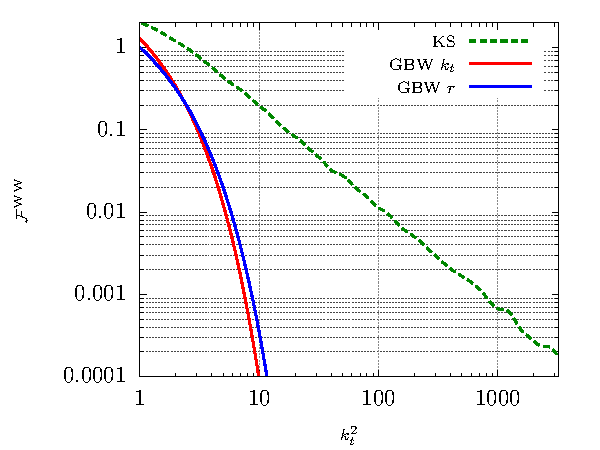
\includegraphics[width=\textwidth]{gnuplot/GBWWW1} 
		\end{subfigure}
		\begin{subfigure}{0.5\textwidth}
			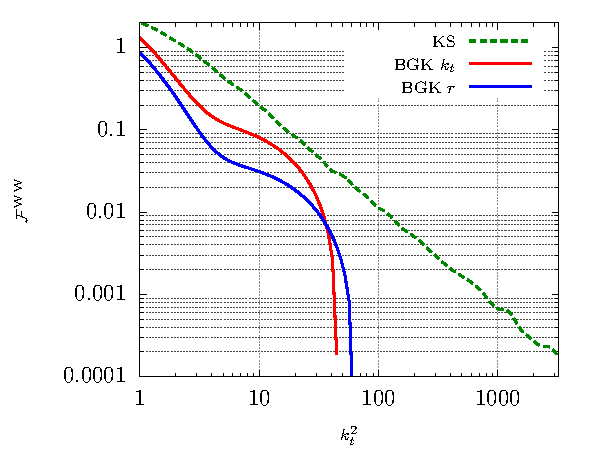
\includegraphics[width=\textwidth]{gnuplot/BGKWW1} 
		\end{subfigure}
		\begin{subfigure}{0.5\textwidth}
			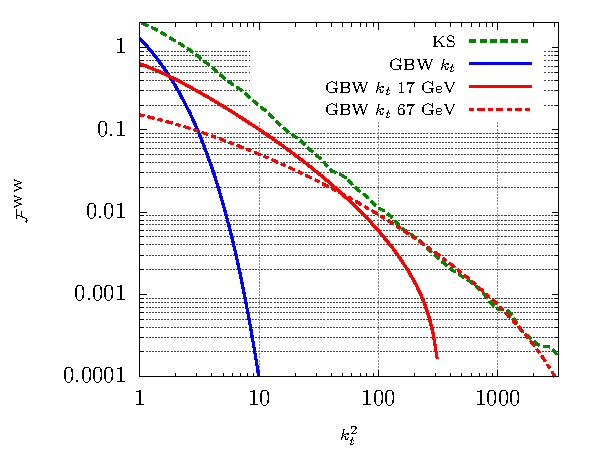
\includegraphics[width=\textwidth]{gnuplot/GBWWW2} 
		\end{subfigure}
		\begin{subfigure}{0.5\textwidth}
			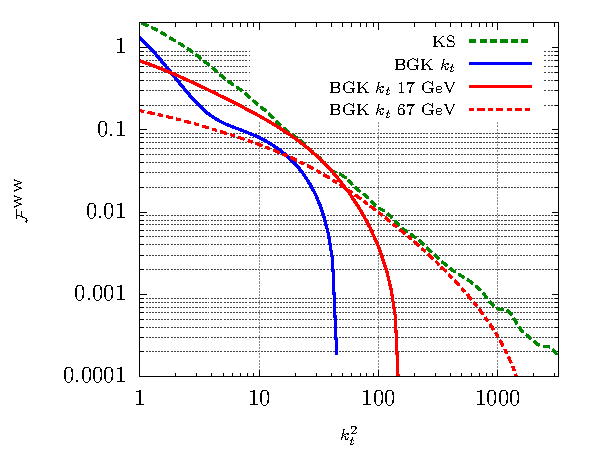
\includegraphics[width=\textwidth]{gnuplot/BGKWW2} 
		\end{subfigure}
		\caption{\footnotesize Weizs\"acker-Williams gluon density at $x=10^{-3}$. Top row: comparison of the dipole-factorization fit and $k_t$-factorization fit results. Bottom row: comparison of the respective models with and without the Sudakov factor, at $\mu=17,\;67 \mathrm{GeV}$. Green dashed line is the KS gluon~\cite{vanHameren:2021sqc}. }
		\label{fig:ww}
	\end{figure}
\section{Dijet process}
In order to investigate less inclusive processes, we will study the electron-dijet correlation at EIC, following closely the method of Ref.~\cite{vanHameren:2021sqc}. 
Dijet process is known to probe a type of unintegrated gluon density, called Weizs\"acker-Williams gluon density~\cite{Dominguez:2010xd,Dominguez:2011wm,Xiao:2017ggh}.
This UGD, $\fww(x,k^2)$, has an interpretation as a number density of gluons inside a proton~\cite{Dominguez:2010xd,Dominguez:2011wm}. Under the Gaussian approximation and assuming $\theta$-like profile of the proton, one can write~\cite{vanHameren:2016ftb,Xiao:2017ggh,Dominguez:2010xd,Dominguez:2011wm}
\begin{equation}
\fww(x,k^2)= \frac{C_F}{2\pi^3\alpha_s}\int^\infty_0\frac{dr}{r}J_0(r k) \sdpa(x,r),
\end{equation} 	
with the adjoint dipole cross section
\begin{equation}
\sdpa(x,r)=\sigma_0\left( 1-\left(1-\frac{\sdp(x,r)}{\sigma_0}\right)^{C_A/C_F}\right).
\label{eq:ww}
\end{equation}
Resummation of the Sudakov logarithms is achieved by the formula~\cite{Xiao:2017yya}
\begin{equation}
	\fww(x,k^2,\mu^2)= \frac{C_F}{2\pi^3\alpha_s}\int^\infty_0\frac{dr}{r}J_0(r k) e^{-S(r,\mu^2)} \sdpa(x,r),
	\label{eq:ww-sud}
\end{equation}
where, we use the Sudakov form factor~\cite{Mueller:2013wwa,Xiao:2017yya},
\begin{equation}
	S(r,\mu^2)=\frac{\alpha_s N_c}{4\pi}\ln^2\left(\frac{\mu^2r^2}{4e^{-2\gamma_E}}\right),
\end{equation}
in which $\gamma_E$ is the Euler-Mascheroni constant, and we use $\alpha_s=0.2$. 
 

  
The present study is carried out in the framework of the small-$x$-Improved Transverse-Momentum-Dependent (ITMD) factorization~\cite{Kotko:2015ura,vanHameren:2016ftb}.
The ITMD factorization is implemented in the program KATIE~\cite{vanHameren:2016kkz}, which we will use to compute the cross section. Important points of the formalism are the following. Firstly, it extends applicability of TMD to the large-$k_t$ region. Thus it recovers the $k_t$-factorization if saturation effects are neglected. Secondly, it is equivalent to CGC, except for lacking multipartonic interaction~(genuine twist)~\cite{Altinoluk:2019fui}. It was discussed in Ref.~\cite{vanHameren:2021sqc}, that with above points and the fact that genuine twists are suppressed when transverse momenta are large \comment{Also, $Q$ but as it was also said, that Q is low here(p.5,\cite{vanHameren:2021sqc}. )  Also it was mentioned the cut on $p_T$ is selected for this. I assume it is $p_{1T}, p_{2T}$ that are relevant?}, ITMD is suitable for studying dijets.

Following Ref.~\cite{vanHameren:2021sqc}, we study the azimuthal correlations of jets and the final state electron in DIS ($e+p\rightarrow e+J_1+J_2+X$), where it was argued that this observable is sensitive to the soft emissions and the saturation effects. 
The kinematical cuts suggested in Ref.~\cite{vanHameren:2021sqc} were
\begin{align*}
	E_e&=15\GeV& E_p&=135\GeV& Q^2&>1\GeV^2\\
	0.1<&\nu<0.85&\Delta R_{\mathrm{Breit}}&<1&p^{\mathrm{Breit}}_{1,2\,T}&>3\GeV\\
	&&-4<&y_{1,2\,\mathrm{lab}}<-1.&&
\end{align*}

Grids of the Weizs\"acker-Williams gluon density were produced by evaluating Eqs.~(\ref{eq:ww}) and~(\ref{eq:ww-sud}).
The gluon density at $x=10^{-3}$ is plotted in Fig.~\ref{fig:ww} with hard-scale-independent KS gluon~\cite{vanHameren:2021sqc}. Clearly, the GBW and BGK models falls much more quickly than the KS gluon density. In general, expected behaviour in the large-$k_t$ region is $\sim k_t^{-2}$~\cite{Dominguez:2010xd,Dominguez:2011wm}, while GBW behaves like $\sim e^{-k_t^2}$.
As in Ref.~\cite{vanHameren:2021sqc}, the Sudakov factor enhances in the small-$k_t$ region and suppresses in the large-$k_t$ region. In comparison to the result of Ref.~\cite{vanHameren:2021sqc}, the effect of broadening by the Sudakov is significantly more pronounced in the case of the GBW and BGK models. The hard-scale-dependent GBW and BGK models, as a consequence, become closer to the KS gluon (also see Fig.~2 of Ref.~\cite{vanHameren:2021sqc}).  

Figs.~\ref{fig:je-breit} and~\ref{fig:je-lab} corresponds to those of Fig.~4 in Ref.~\cite{vanHameren:2021sqc} ($e$-jets azimuthal correlation). 
In the top row of Fig.~\ref{fig:je-breit}, we clearly see, for both the GBW and BGK models, better agreements of results with the KS for the new $k_t$-factorization fits. In the middle and the bottom row, it shows the effects of the Sudakov form factor, which qualitatively agrees with that of Ref.~\cite{vanHameren:2021sqc}, by lowering the cross section.
Fig.~\ref{fig:je-lab} shows the $e$-jets correlation in the lab frame. Here, the difference between KS and GBW and BGK are more prominent. Unlike in the previous plots, the new fits in the $k_t$-factorization shows only limited improvement.
The effects of the Sudakov factor is similar to those in Ref.~\cite{vanHameren:2021sqc} at relatively high $\Delta \phi$, while at smaller $\Delta \phi$ region the effect is reversed (i.e. The cross sections were slightly lowered in Ref.~\cite{vanHameren:2021sqc}, while here, they are significantly increased). \comment{probably related to the high $k_t$ region of the gluon density?}\\
\comment{regarding this differences between Breit and lab frames, what does "\dots since it (breit) suppresses the LO contributions, i.e. process dominated by a quark jet." mean?}

\begin{figure}[p]
	\begin{subfigure}{0.5\textwidth}
	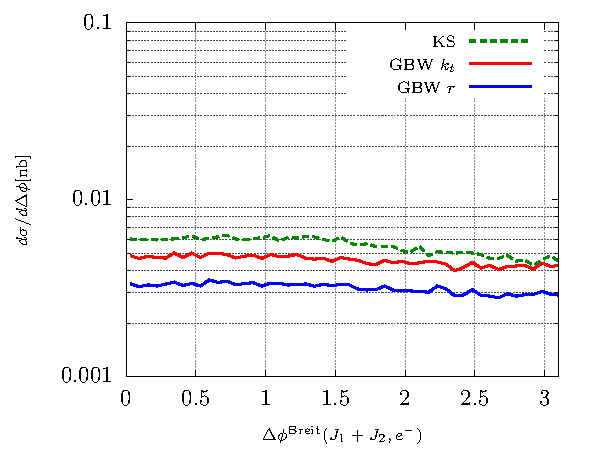
\includegraphics[width=\textwidth]{gnuplot/plotGBW1} 
	\end{subfigure}
	\begin{subfigure}{0.5\textwidth}
	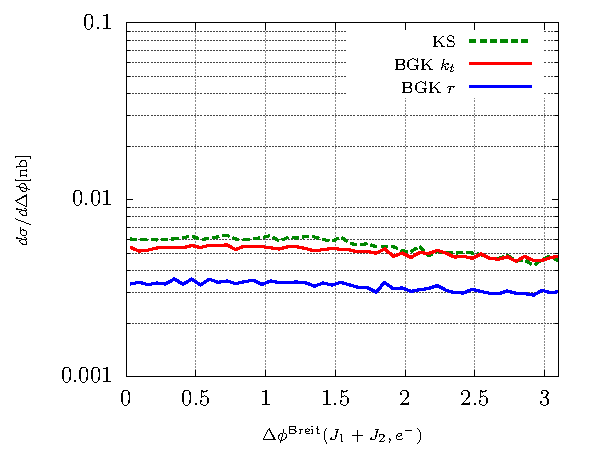
\includegraphics[width=\textwidth]{gnuplot/plotBGK1} 
	\end{subfigure}
%	\caption{ }
%\end{figure}
%\begin{figure}[t]
	\begin{subfigure}{0.5\textwidth}
	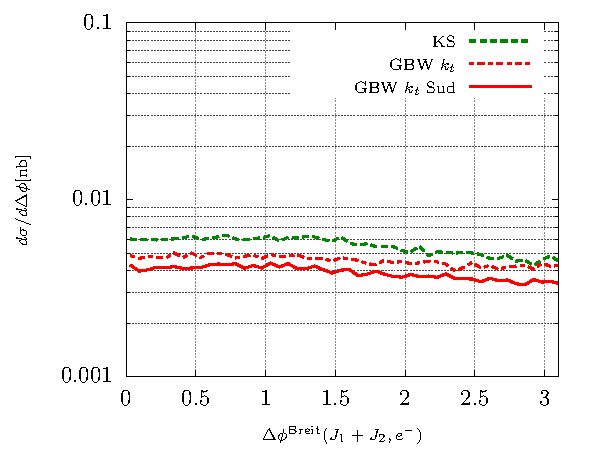
\includegraphics[width=\textwidth]{gnuplot/plotGBW2}
	\end{subfigure}
	\begin{subfigure}{0.5\textwidth}
	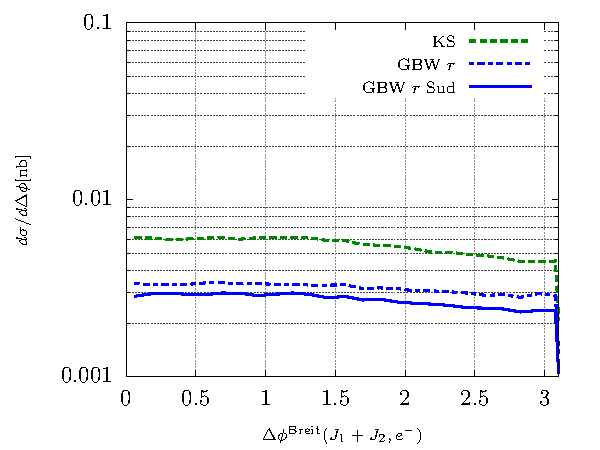
\includegraphics[width=\textwidth]{gnuplot/plotGBW3}
	\end{subfigure}
	\begin{subfigure}{0.5\textwidth}
	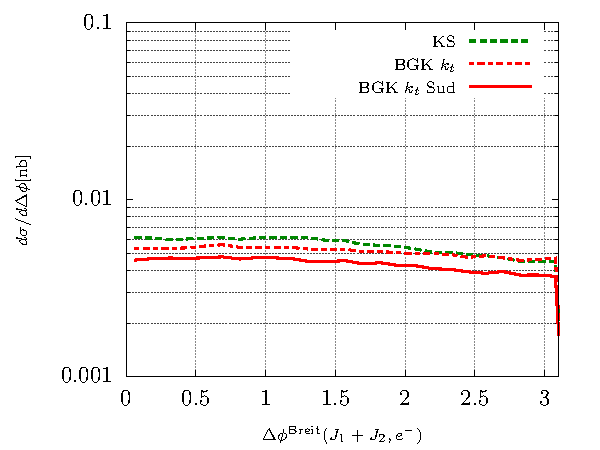
\includegraphics[width=\textwidth]{gnuplot/plotBGK2}
	\end{subfigure}
	\begin{subfigure}{0.5\textwidth}
	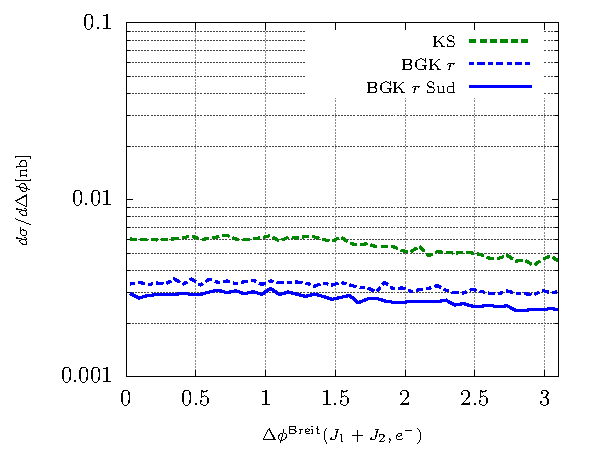
\includegraphics[width=\textwidth]{gnuplot/plotBGK3}
	\end{subfigure}
	\caption{\footnotesize Azimuthal correlation of the jets and the scattered electron in the Breit frame. Top: Comparison of dipole-factorization fit and $k_t$-factorization fit. Middle \& Bottom: Effect of the Sudakov form factor.   Green dashed line is the KS gluon~\cite{vanHameren:2021sqc}.}
	\label{fig:je-breit}
\end{figure}

\begin{figure}[p]
	\begin{subfigure}{0.5\textwidth}
		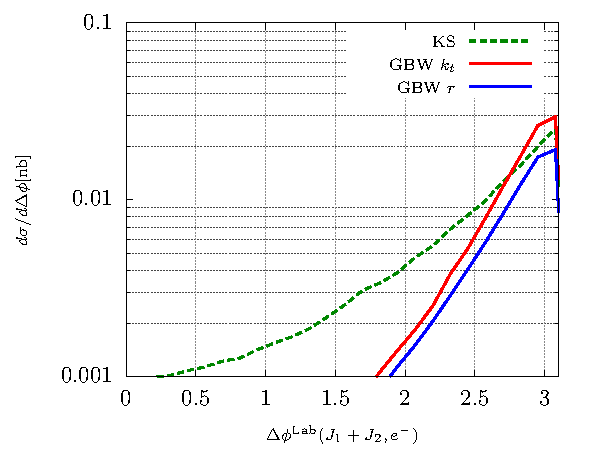
\includegraphics[width=\textwidth]{gnuplot/plotGBW1Lab} 
	\end{subfigure}
	\begin{subfigure}{0.5\textwidth}
		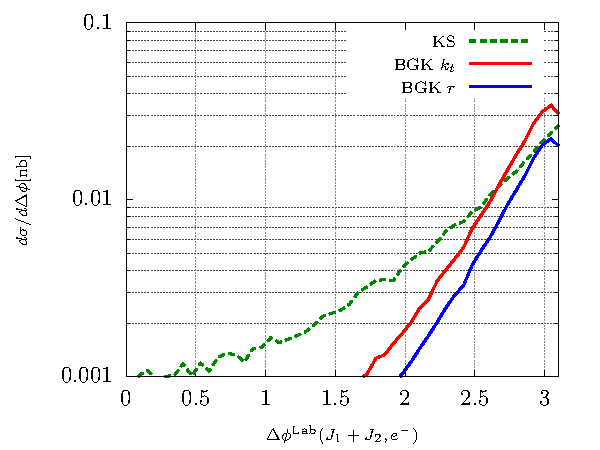
\includegraphics[width=\textwidth]{gnuplot/plotBGK1Lab} 
	\end{subfigure}
	\begin{subfigure}{0.5\textwidth}
		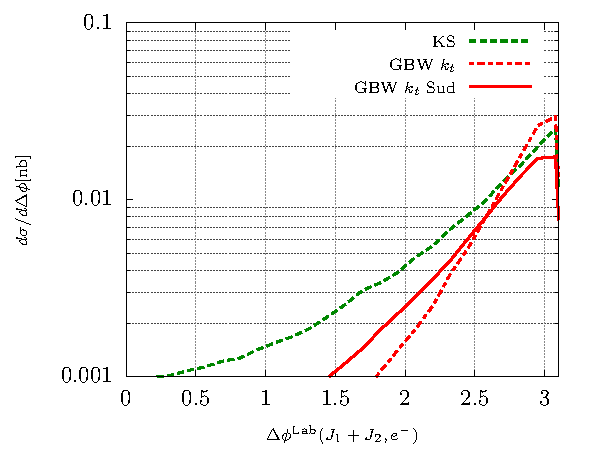
\includegraphics[width=\textwidth]{gnuplot/plotGBW2Lab}
	\end{subfigure}
	\begin{subfigure}{0.5\textwidth}
		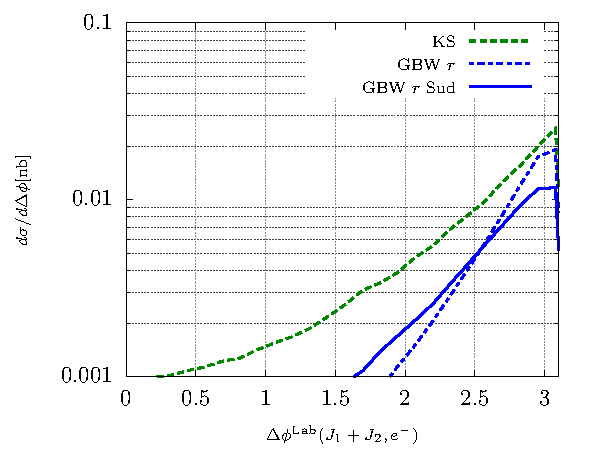
\includegraphics[width=\textwidth]{gnuplot/plotGBW3Lab}
	\end{subfigure}
	\begin{subfigure}{0.5\textwidth}
		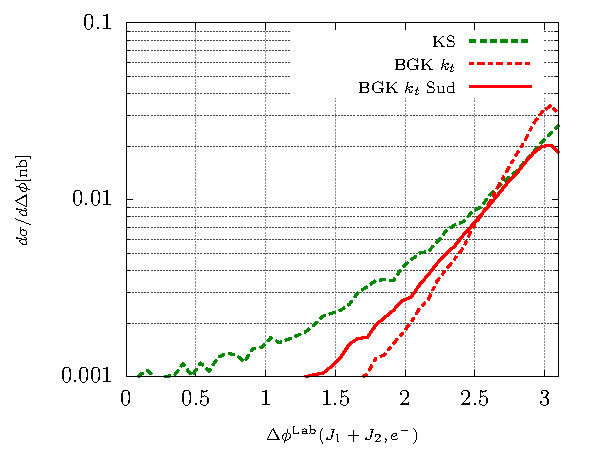
\includegraphics[width=\textwidth]{gnuplot/plotBGK2Lab}
	\end{subfigure}
	\begin{subfigure}{0.5\textwidth}
		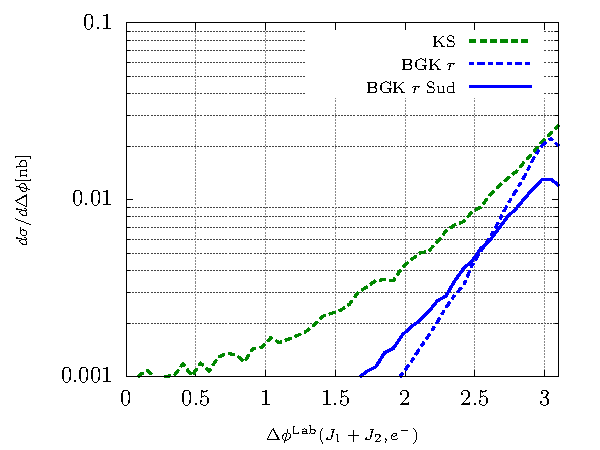
\includegraphics[width=\textwidth]{gnuplot/plotBGK3Lab}
	\end{subfigure}
\caption{\footnotesize Azimuthal correlation of the jets and the scattered electron in the lab frame. Top: Comparison of dipole-factorization fit and $k_t$-factorization fit. Middle \& Bottom: Effect of the Sudakov form factor.  Green dashed line is the KS gluon~\cite{vanHameren:2021sqc}.}
\label{fig:je-lab}
\end{figure}

Finally, Fig.~\ref{fig:jj-breit} shows the jet correlations in the Breit frame. Again, the GBW and BGK models show considerable deviation from the KS gluon. Similarly to the previous plots, the Sudakov factor affects the models differently from the KS in Ref.~\cite{vanHameren:2021sqc}.
The effect enhances the cross section considerably in the small-$\Delta\phi$ region, making it closer to KS gluon result.
%The result seems natural as small $k_t$ corresponds to the back-to-back configuration of the jets, and as it can be seen clearly in Fig.~\ref{fig:ww}, the GBW and BGK gluons are much lower than the KS gluon. 

\begin{figure}[p]
	\begin{subfigure}{0.48\textwidth}
		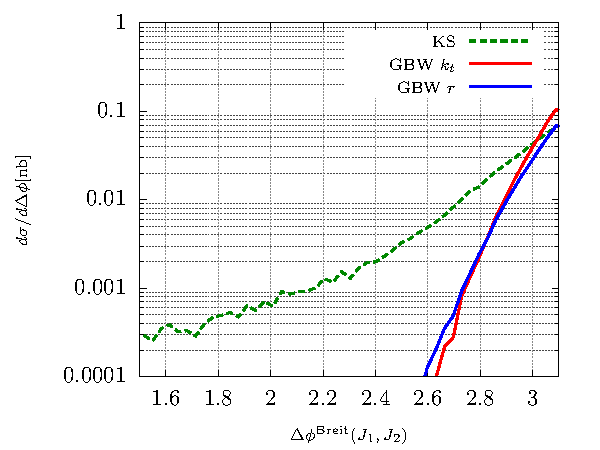
\includegraphics[width=\textwidth]{gnuplot/plotGBW1Jets} 
	\end{subfigure}
	\begin{subfigure}{0.48\textwidth}
		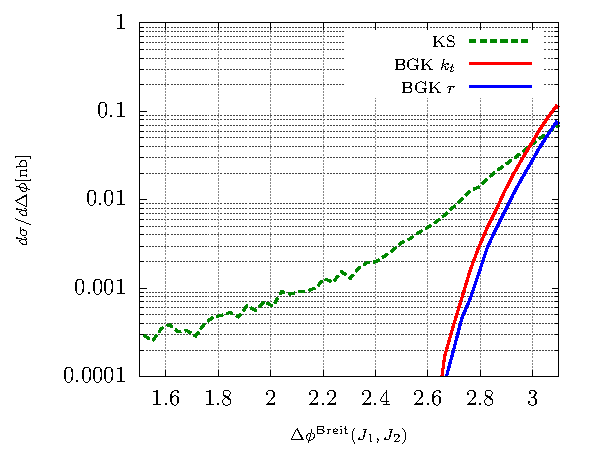
\includegraphics[width=\textwidth]{gnuplot/plotBGK1Jets} 
	\end{subfigure}
	\begin{subfigure}{0.48\textwidth}
		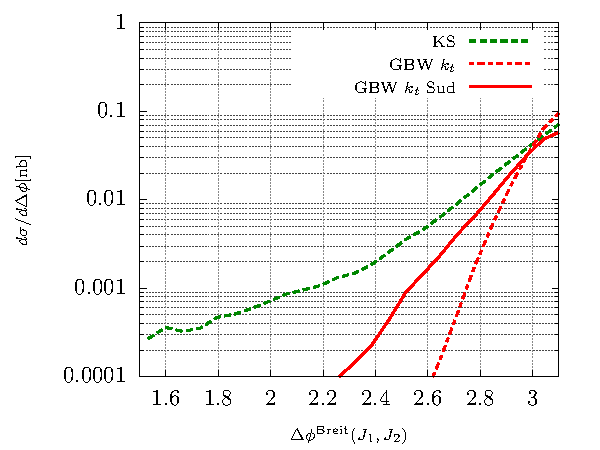
\includegraphics[width=\textwidth]{gnuplot/plotGBW2Jets}
	\end{subfigure}
	\begin{subfigure}{0.48\textwidth}
		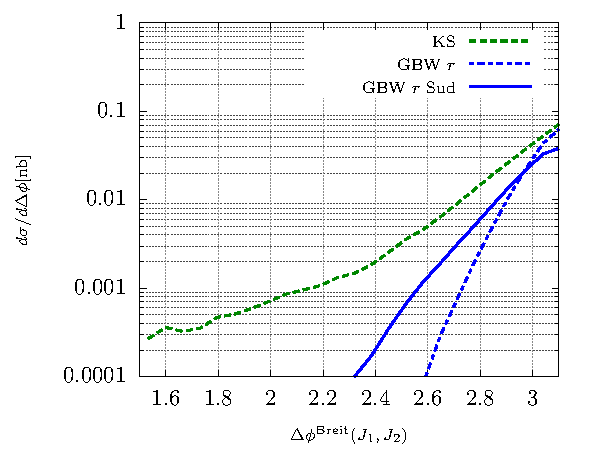
\includegraphics[width=\textwidth]{gnuplot/plotGBW3Jets}
	\end{subfigure}
	\begin{subfigure}{0.48\textwidth}
		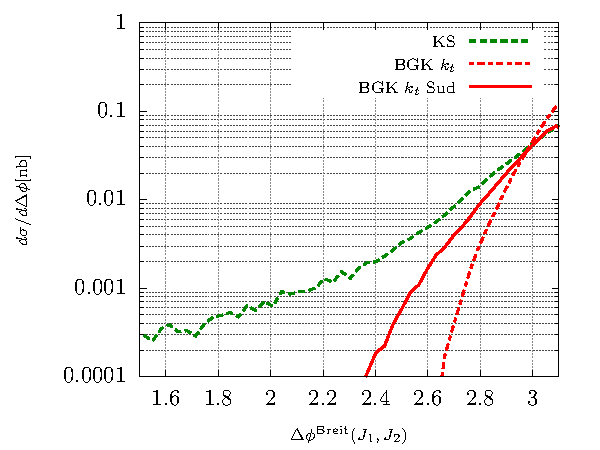
\includegraphics[width=\textwidth]{gnuplot/plotBGK2Jets}
	\end{subfigure}
	\begin{subfigure}{0.48\textwidth}
		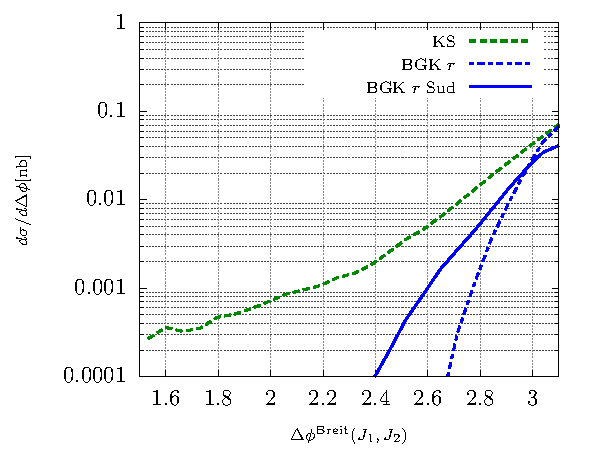
\includegraphics[width=\textwidth]{gnuplot/plotBGK3Jets}
	\end{subfigure}
\caption{\footnotesize Azimuthal correlation of the jets in the Breit frame. Top: Comparison of dipole-factorization fit and $k_t$-factorization fit. Middle \& Bottom: Effect of the Sudakov form factor. Green dashed line is the KS gluon~\cite{vanHameren:2021sqc}. }
\label{fig:jj-breit}
\end{figure}



\appendix	
\section{Computation of gluon densities}
In the evaluation Eq.~(\ref{eq:ww}) the convergence of this integral may be slow due to high oscillation for large $k$.
For such integration, one can employ a method summarized in Ref.~\cite{LYNESS1985109}. 
Essentially, the integration is carried out between, anti-nodes of $J_0(rk)$. Then the total integral is written in the form of infinite sum
\begin{equation}
	I=\sum^\infty_{i=1} \int^{a_{i+1}}_{a_i} \frac{dr}{r}J_0(r k) \sdpa(x,r),
\end{equation}
where we use $a_{i}=\frac{\pi}{k}(i+1/4)$.
This sum can be accelerated, with series transformation described in Ref.~\cite{doi:10.1080/00207167308803075,Weniger:1989rea,HOMEIER19951}.
The remarkable power of the Levin's transformation is shown in Tab.~\ref{tab:levin}.
This trick is also useful in the computation of dipole gluon density. 

\begin{table}
	\begin{center}
		\begin{tabular}{|c||c|c|}
			\hline
			$n$&Levin&Sum\\\hline
			9&	-5.751e-9&	-0.0004998\\\hline
			12&	-1.5891e-9&	0.00025567\\\hline
			15&	-3.803e-11&	-0.00015069\\\hline
			18&	6.639e-13&	0.00009743\\\hline
			21&	2.6728e-13&	-0.00006722\\\hline
			24&	2.6744e-13&	0.00004866\\\hline
			27&	2.6744e-13&	-0.00003655\\\hline
		\end{tabular}
	\end{center}
	\caption{
		Computing $\int \frac{dr}{r}J_0(r k)(1-e^{-r^2})$, with $k=10$ adding up to $n$ th term.
		Levin-accelerated case reaches the true value of $\sim$2.674e-13 far more quickly, and shows superior stability.
	}
	\label{tab:levin}
\end{table}
\printbibliography
\end{document}


